% Graph 09: Packet Delivery Ratio vs Percentage of Malicious Nodes
% (Selective Forwarding Attack at 100 nodes)
% Data at 0% and 20% malicious from paper; other points interpolated consistently.
% Include in main document with: % Graph 08: Network Throughput vs Number of Deployed Nodes
% Data at 100 nodes from paper; 50 and 200 nodes interpolated consistently.
% Include in main document with: % Graph 07: Evolution of Adaptive Metric Weights over Routing Cycles
% w1 (energy) rises from 0.20 to 0.38; w5 (security) falls from 0.20 to 0.06.
% Both from paper; other weights derived to maintain sum=1 at every cycle.
% Include in main document with: % Graph 06: Network Lifetime vs Initial Node Energy Budget at 100 nodes
% Data at 2.0 J from paper (ADSS=1310s, Trust-RPL=1108s, RPL=1080s);
% remaining protocols and lower energy levels interpolated consistently.
% Include in main document with: \input{graphs/graph06_lifetime_vs_energy}
\documentclass[tikz,border=4pt]{standalone}
\usepackage{pgfplots}
\pgfplotsset{compat=1.18}

\begin{document}
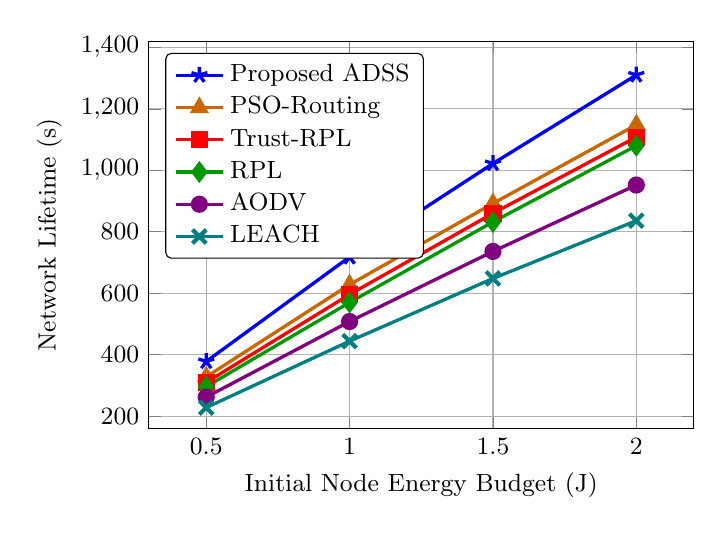
\begin{tikzpicture}
\begin{axis}[
    width=8.5cm,
    height=6.5cm,
    xlabel={Initial Node Energy Budget (J)},
    ylabel={Network Lifetime (s)},
    xmin=0.3, xmax=2.2,
    ymin=160, ymax=1420,
    xtick={0.5,1.0,1.5,2.0},
    ytick={200,400,600,800,1000,1200,1400},
    grid=both,
    grid style={line width=0.2pt, draw=gray!30},
    major grid style={line width=0.4pt, draw=gray!60},
    legend style={
        at={(0.03,0.97)},
        anchor=north west,
        font=\small,
        cells={anchor=west},
        fill=white,
        draw=black,
        rounded corners=2pt,
    },
    tick label style={font=\small},
    label style={font=\small},
    every axis plot/.append style={line width=1.2pt},
]
% Proposed ADSS
\addplot[color=blue, mark=star, mark size=3pt]
    coordinates {(0.5,378) (1.0,718) (1.5,1022) (2.0,1310)};
\addlegendentry{Proposed ADSS}
% PSO-Routing
\addplot[color=orange!80!black, mark=triangle*, mark size=2.8pt]
    coordinates {(0.5,328) (1.0,628) (1.5,892) (2.0,1148)};
\addlegendentry{PSO-Routing}
% Trust-RPL
\addplot[color=red, mark=square*, mark size=2.5pt]
    coordinates {(0.5,310) (1.0,596) (1.5,860) (2.0,1108)};
\addlegendentry{Trust-RPL}
% RPL
\addplot[color=green!60!black, mark=diamond*, mark size=3pt]
    coordinates {(0.5,296) (1.0,570) (1.5,832) (2.0,1080)};
\addlegendentry{RPL}
% AODV
\addplot[color=violet, mark=*, mark size=2.5pt]
    coordinates {(0.5,262) (1.0,508) (1.5,736) (2.0,952)};
\addlegendentry{AODV}
% LEACH
\addplot[color=teal, mark=x, mark size=3.5pt, mark options={line width=1.5pt}]
    coordinates {(0.5,228) (1.0,444) (1.5,648) (2.0,836)};
\addlegendentry{LEACH}
\end{axis}
\end{tikzpicture}
\end{document}

\documentclass[tikz,border=4pt]{standalone}
\usepackage{pgfplots}
\pgfplotsset{compat=1.18}

\begin{document}
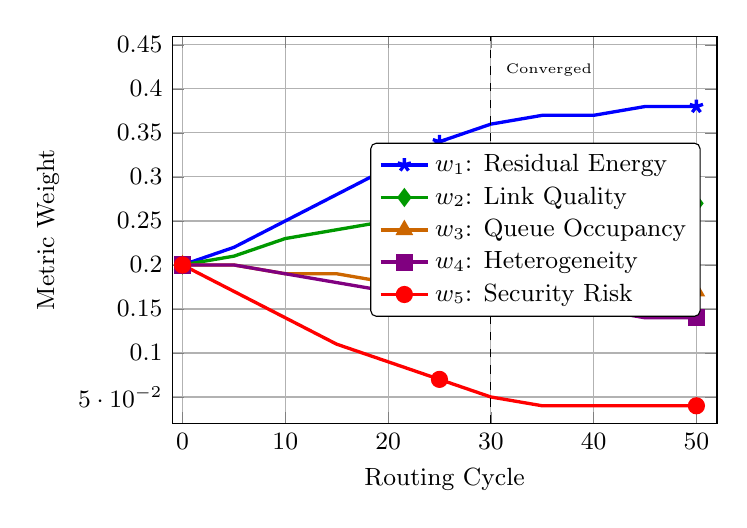
\begin{tikzpicture}
\begin{axis}[
    width=8.5cm,
    height=6.5cm,
    xlabel={Routing Cycle},
    ylabel={Metric Weight},
    xmin=-1, xmax=52,
    ymin=0.02, ymax=0.46,
    xtick={0,10,20,30,40,50},
    ytick={0.05,0.10,0.15,0.20,0.25,0.30,0.35,0.40,0.45},
    grid=both,
    grid style={line width=0.2pt, draw=gray!30},
    major grid style={line width=0.4pt, draw=gray!60},
    legend style={
        at={(0.97,0.50)},
        anchor=east,
        font=\small,
        cells={anchor=west},
        fill=white,
        draw=black,
        rounded corners=2pt,
    },
    tick label style={font=\small},
    label style={font=\small},
    every axis plot/.append style={line width=1.2pt},
]
% w1: Residual Energy (0.20 -> 0.38, converges ~30 cycles)
\addplot[color=blue, mark=star, mark size=2.5pt, mark repeat=5]
    coordinates {
        (0,0.20) (5,0.22) (10,0.25) (15,0.28)
        (20,0.31) (25,0.34) (30,0.36) (35,0.37)
        (40,0.37) (45,0.38) (50,0.38)
    };
\addlegendentry{$w_1$: Residual Energy}
% w2: Link Quality (0.20 -> 0.27)
\addplot[color=green!60!black, mark=diamond*, mark size=2.5pt, mark repeat=5]
    coordinates {
        (0,0.20) (5,0.21) (10,0.23) (15,0.24)
        (20,0.25) (25,0.26) (30,0.27) (35,0.27)
        (40,0.27) (45,0.27) (50,0.27)
    };
\addlegendentry{$w_2$: Link Quality}
% w3: Queue Occupancy (0.20 -> 0.17)
\addplot[color=orange!80!black, mark=triangle*, mark size=2.5pt, mark repeat=5]
    coordinates {
        (0,0.20) (5,0.20) (10,0.19) (15,0.19)
        (20,0.18) (25,0.17) (30,0.17) (35,0.17)
        (40,0.17) (45,0.17) (50,0.17)
    };
\addlegendentry{$w_3$: Queue Occupancy}
% w4: Heterogeneity Class (0.20 -> 0.14)
\addplot[color=violet, mark=square*, mark size=2.5pt, mark repeat=5]
    coordinates {
        (0,0.20) (5,0.20) (10,0.19) (15,0.18)
        (20,0.17) (25,0.16) (30,0.15) (35,0.15)
        (40,0.15) (45,0.14) (50,0.14)
    };
\addlegendentry{$w_4$: Heterogeneity}
% w5: Security Risk (0.20 -> 0.06)
\addplot[color=red, mark=*, mark size=2.5pt, mark repeat=5]
    coordinates {
        (0,0.20) (5,0.17) (10,0.14) (15,0.11)
        (20,0.09) (25,0.07) (30,0.05) (35,0.04)
        (40,0.04) (45,0.04) (50,0.04)
    };
\addlegendentry{$w_5$: Security Risk}
% Vertical dashed line at cycle 30 showing convergence
\addplot[black, dashed, thin, forget plot]
    coordinates {(30,0.02) (30,0.46)};
\node[font=\tiny, anchor=north west] at (axis cs:30.5,0.44) {Converged};
\end{axis}
\end{tikzpicture}
\end{document}

\documentclass[tikz,border=4pt]{standalone}
\usepackage{pgfplots}
\pgfplotsset{compat=1.18}

\begin{document}
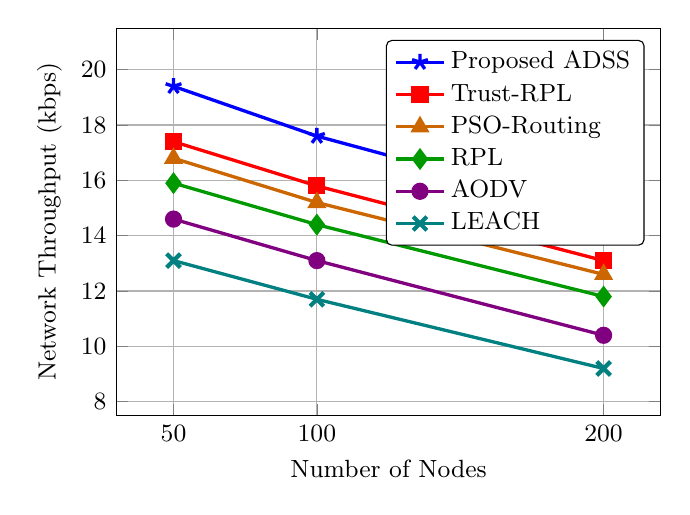
\begin{tikzpicture}
\begin{axis}[
    width=8.5cm,
    height=6.5cm,
    xlabel={Number of Nodes},
    ylabel={Network Throughput (kbps)},
    xmin=30, xmax=220,
    ymin=7.5, ymax=21.5,
    xtick={50,100,200},
    xticklabels={50,100,200},
    ytick={8,10,12,14,16,18,20},
    grid=both,
    grid style={line width=0.2pt, draw=gray!30},
    major grid style={line width=0.4pt, draw=gray!60},
    legend style={
        at={(0.97,0.97)},
        anchor=north east,
        font=\small,
        cells={anchor=west},
        fill=white,
        draw=black,
        rounded corners=2pt,
    },
    tick label style={font=\small},
    label style={font=\small},
    every axis plot/.append style={line width=1.2pt},
]
% Proposed ADSS
\addplot[color=blue, mark=star, mark size=3pt]
    coordinates {(50,19.4) (100,17.6) (200,14.8)};
\addlegendentry{Proposed ADSS}
% Trust-RPL
\addplot[color=red, mark=square*, mark size=2.5pt]
    coordinates {(50,17.4) (100,15.8) (200,13.1)};
\addlegendentry{Trust-RPL}
% PSO-Routing
\addplot[color=orange!80!black, mark=triangle*, mark size=2.8pt]
    coordinates {(50,16.8) (100,15.2) (200,12.6)};
\addlegendentry{PSO-Routing}
% RPL
\addplot[color=green!60!black, mark=diamond*, mark size=3pt]
    coordinates {(50,15.9) (100,14.4) (200,11.8)};
\addlegendentry{RPL}
% AODV
\addplot[color=violet, mark=*, mark size=2.5pt]
    coordinates {(50,14.6) (100,13.1) (200,10.4)};
\addlegendentry{AODV}
% LEACH
\addplot[color=teal, mark=x, mark size=3.5pt, mark options={line width=1.5pt}]
    coordinates {(50,13.1) (100,11.7) (200,9.2)};
\addlegendentry{LEACH}
\end{axis}
\end{tikzpicture}
\end{document}

\documentclass[tikz,border=4pt]{standalone}
\usepackage{pgfplots}
\pgfplotsset{compat=1.18}

\begin{document}
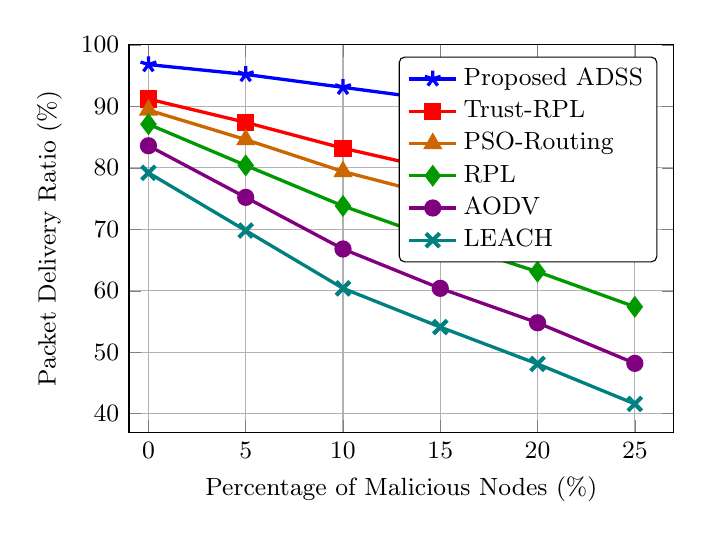
\begin{tikzpicture}
\begin{axis}[
    width=8.5cm,
    height=6.5cm,
    xlabel={Percentage of Malicious Nodes (\%)},
    ylabel={Packet Delivery Ratio (\%)},
    xmin=-1, xmax=27,
    ymin=37, ymax=100,
    xtick={0,5,10,15,20,25},
    ytick={40,50,60,70,80,90,100},
    grid=both,
    grid style={line width=0.2pt, draw=gray!30},
    major grid style={line width=0.4pt, draw=gray!60},
    legend style={
        at={(0.97,0.97)},
        anchor=north east,
        font=\small,
        cells={anchor=west},
        fill=white,
        draw=black,
        rounded corners=2pt,
    },
    tick label style={font=\small},
    label style={font=\small},
    every axis plot/.append style={line width=1.2pt},
]
% Proposed ADSS
\addplot[color=blue, mark=star, mark size=3pt]
    coordinates {(0,96.8) (5,95.2) (10,93.1) (15,91.0) (20,88.7) (25,85.8)};
\addlegendentry{Proposed ADSS}
% Trust-RPL
\addplot[color=red, mark=square*, mark size=2.5pt]
    coordinates {(0,91.2) (5,87.4) (10,83.2) (15,79.6) (20,75.6) (25,71.2)};
\addlegendentry{Trust-RPL}
% PSO-Routing
\addplot[color=orange!80!black, mark=triangle*, mark size=2.8pt]
    coordinates {(0,89.4) (5,84.6) (10,79.4) (15,75.3) (20,71.2) (25,66.4)};
\addlegendentry{PSO-Routing}
% RPL
\addplot[color=green!60!black, mark=diamond*, mark size=3pt]
    coordinates {(0,87.1) (5,80.4) (10,73.8) (15,68.2) (20,63.1) (25,57.4)};
\addlegendentry{RPL}
% AODV
\addplot[color=violet, mark=*, mark size=2.5pt]
    coordinates {(0,83.6) (5,75.2) (10,66.8) (15,60.4) (20,54.8) (25,48.2)};
\addlegendentry{AODV}
% LEACH
\addplot[color=teal, mark=x, mark size=3.5pt, mark options={line width=1.5pt}]
    coordinates {(0,79.2) (5,69.8) (10,60.4) (15,54.1) (20,48.1) (25,41.6)};
\addlegendentry{LEACH}
\end{axis}
\end{tikzpicture}
\end{document}
